\documentclass{article}
\usepackage[utf8]{inputenc}
\usepackage{indentfirst}
\setlength{\parindent}{1em}
\usepackage{graphicx} 
\usepackage{geometry}

\geometry{a4paper,scale=0.8}


\title{The Clonal Selection Algorithm}
\author{CaoJing \quad 21721243}
\date{April 2018}

\begin{document}

\maketitle

\section{The Clonal Selection Theory}
When an animal is exposed to an antigen, some subpopulation of its bone marrow derived cells (B lymphocytes) respond by producing antibodies (\textbf{Ab}). Each cell secretes only one kind of antibody, which is relatively specific for the antigen. By binding to these antibodies (receptors), and with a second signal from accessory cells, such as the T-helper cell, the antigen stimulates the B cell to proliferate (divide) and mature into terminal (non-dividing) antibody secreting cells, called plasma cells. The various cell divisions (mitosis) generate a clone, i.e., a set of cells that are the progeny of a single cell. While plasma cells are the most active antibody secretors, large B lymphocytes, which divide rapidly, also secrete \textbf{Ab}, albeit at a lower rate. While B cells secrete \textbf{Ab}, T cells play a central role in the regulation of the B cell response and are preeminent in cell mediated immune responses.

Lymphocytes, in addition to proliferating and/or differentiating into plasma cells, can differentiate into long-lived B memory cells. Memory cells circulate through the blood, lymph and tissues, and when exposed to a second antigenic stimulus commence to differentiate into large lymphocytes capable of producing high affinity antibodies, pre-selected for the specific antigen that had stimulated the primary response. Figure 1 depicts the clonal selection principle.

The main features of the clonal selection theory are:
\begin{itemize}
\item{generation of new random genetic changes, subsequently expressed as diverse antibody patterns by a form of accelerated somatic mutation;}
\item{phenotypic restriction and retention of one pattern to one differentiated cell (clone);}
\item{proliferation and differentiation on contact of cells
with antigens.}
\end{itemize}

\begin{center} 
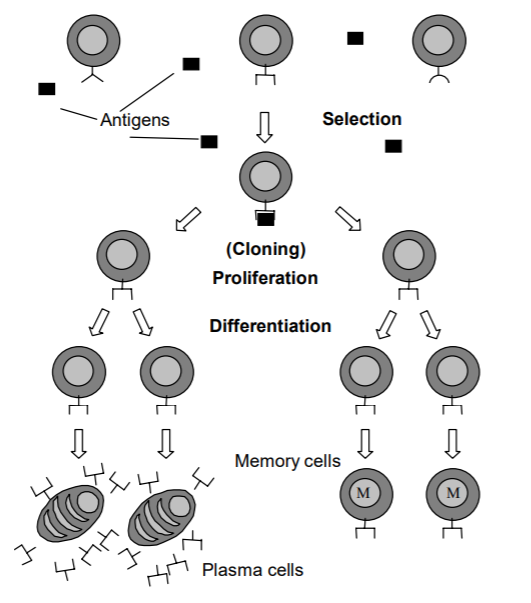
\includegraphics[width=8cm,clip]{images/cj_clone_selection_p.png}\\
\caption{Figure 1: The clonal selection principle.}	
\end{center} 


\section{Reinforcement Learning and Memory}
In the normal course of the immune system evolution, an organism would be expected to encounter a given antigen repeatedly during its life time. The initial exposure to an antigen that stimulates an adaptive immune response is handled by a spectrum of small clones of B cells each producing antibody of different affinity. The effectiveness of the immune response to secondary encounters is considerably enhanced by storing some high affinity antibody producing cells from the first infection (memory cells), so as to form a large initial improved clone for subsequent encounters. Rather than ‘starting from scratch’ every time, such a strategy ensures that both the speed and accuracy of the immune response becomes successively greater after each infection. This scheme is intrinsic of a \textsl{reinforcement learning strategy}, where the system is continuously improving its capability to perform its task.

One important characteristic of the immune memory is that it is associative: B cells adapted to a certain type of antigen A1 presents a faster and more efficient secondary response not only to A1, but also to any structurally related antigen A2. This phenomenon is called \textsl{immunological cross-reaction}, or \textsl{cross-reactive response}. Figure 2 depicts the scenario.

\begin{center} 
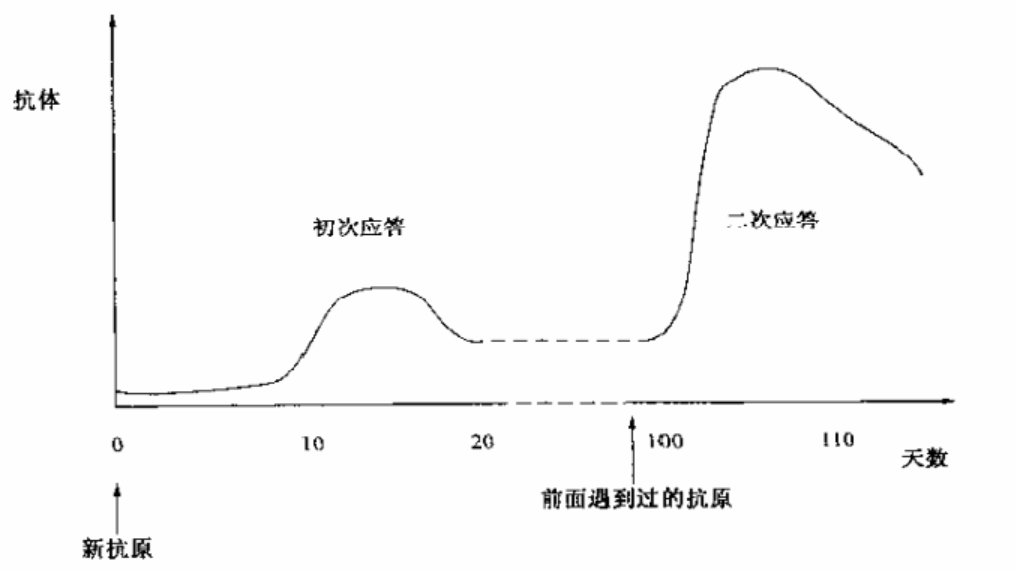
\includegraphics[width=8cm,clip]{images/cj_reinfor_learn.png}\\
\caption{Figure 2: The reinforcement learning.}	
\end{center} 


\section{Somatic Hypermutation, Receptor Editing and Repertoire Diversity}
In a T cell dependent immune response, the repertoire of antigen-activated B cells is diversified basically by two mechanisms: \textsl{hypermutation} and \textsl{receptor editing}.

Random changes are introduced into the genes responsible for the \textbf{Ag-Ab} interactions and occasionally one such change will lead to an increase in the affinity of the antibody. It is these high-affinity variants which are then selected to enter the pool of memory cells. Not only the repertoire is diversified through a hypermutation mechanism, but also mechanisms must exist such that rare B cells with high affinity mutant receptors can be selected to dominate the response. Those cells with low affinity receptors must be efficiently eliminated, become anergic or be edited, so that they do not significantly contribute to the pool of memory cells.

So, in short, the mutation mechanism can be conclude into two points as below. Figure 3 depicts the scenario.

\begin{itemize}
\item{Point mutations allow the immune system to explore
local areas around A by making small steps towards an antibody with higher affinity;}

\item{Receptor editing allows an antibody to take large
steps through the landscape, landing in a locale where the affinity might be lower;}
\end{itemize}

\begin{center} 
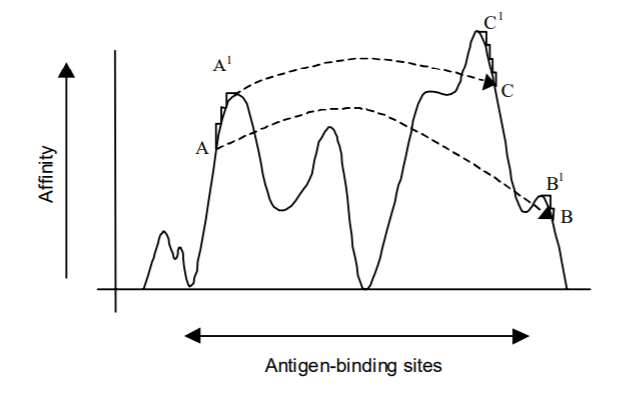
\includegraphics[width=8cm,clip]{images/cj_somatic_muta.png}\\
\caption{Figure 3: Schematic representation of shape-space for antigen-binding sites. Somatic mutations guide to local optima, while receptor editing introduce diversity, leading to possibly better candidate receptors.}	
\end{center} 


\section{The Shape-Space Model}
The shape-space model (S) aims at quantitatively describing the interactions among antigens and antibodies (\textbf{Ag-Ab}). The set of features that characterize a molecule
is called its generalized shape. The Ag-Ab representation (binary or real-valued) determines a distance measure to be used to calculate the degree of interaction between these molecules.  Mathematically, the generalized shape of a molecule (\begin{math} m\end{math}), either an antibody or an antigen, can be represented by a set of coordinates \begin{math} m =\left \langle m_1, m_2,..., m_L\right\rangle\end{math}, which can be regarded as a point in an L-dimensional real-valued shape-space (m \in S^L).

\section{The Proposed Algorithm}
After discussing the clonal selection principle and the affinity maturation process, the development of the clonal selection algorithm (CSA) is straightforward. The main immune aspects taken into account were: maintenance of the memory cells functionally disconnected from the repertoire, selection and cloning of the most stimulated cells, death of non-stimulated cells, affinity maturation and re-selection of the clones with higher affinity, generation and maintenance of diversity, hypermutation proportional to the cell affinity.

The algorithm works as in Figure 4 (after each six steps we have one cell generation):

\begin{center} 
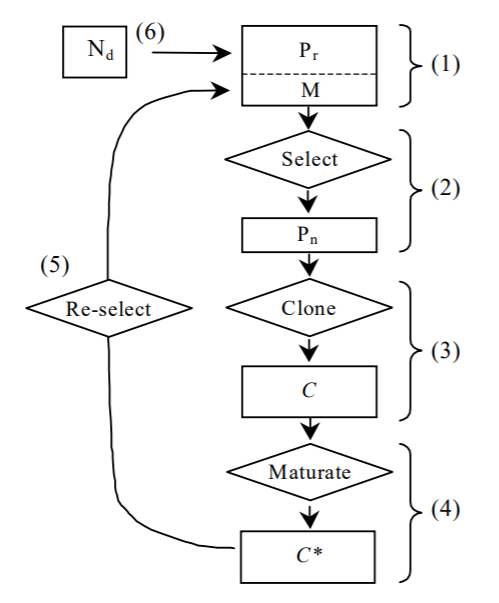
\includegraphics[width=8cm,clip]{images/cj_block_diagram_CSA.png}\\
\caption{Figure 4: Block diagram of the clonal selection algorithm.}	
\end{center} 

\begin{itemize}
\item{(1) Generate a set of (\begin{math} P \end{math}) of candidate solutions, composed of the subset of memory cells  (\begin{math} M \end{math}) added to the remaining (\begin{math} P_r \end{math}) population (\begin{math} P = P_r + M \end{math});}
\item{(2) Determine (Select) the n best individuals of population (\begin{math} P_n \end{math}), based on affinity measure;}
\item{(3) Reproduce (Clone) these n best individuals of the population, giving rise to a temporary population of clones (\begin{math} C \end{math}). The clone size is an increasing function of the affinity with the antigen;}
\item{(4) Submit the population of clones to a hypermutation scheme, where the hypermutation is proportional to the affinity of the antibody with the antigen. A maturated antibody population is generated (\begin{math} C^* \end{math});}
\item{(5) Re-select the improved individuals from \begin{math} C^* \end{math} to compose the memory set \begin{math} M \end{math}. Some members of \begin{math} P \end{math} can be replaced by other improved members of \begin{math} C^* \end{math};}
\item{(6) Replace \begin{math} d \end{math} antibodies by novel ones (diversity introduction). The lower affinity cells have higher probabilities of being replaced;}

\end{itemize}

\section{Engineering Applications}
\subsection{Binary Character Recognition}
The goal is to demonstrate that a cumulative blind variation together with selection can produce individuals with increasing affinities (maturation of the immune response). In this case, we assume that the antigen population is represented by a set of eight binary characters to be learned. Each character is represented by a bitstring of length \begin{math} L = 120 \end{math}.

The affinity measure takes into account the Hamming distance (\begin{math} D \end{math}) between antigens and antibodies, according to Equation (1):
\begin{equation} \small{
D =\sum_{i=1}^{L} \delta \quad where \  \delta = \begin{cases} 1 & \mbox{ if } \  ab_i \neq ag_i \\
0  & otherwise \end{cases}}
 \end{equation}

The original characters (antigens) are depicted in Figure 5(a). Figure 5(b) illustrates the initial memory set, and Figures 5(b) to 5(e) represent the maturation of the memory set (immune response) through cell generations.

\begin{center} 
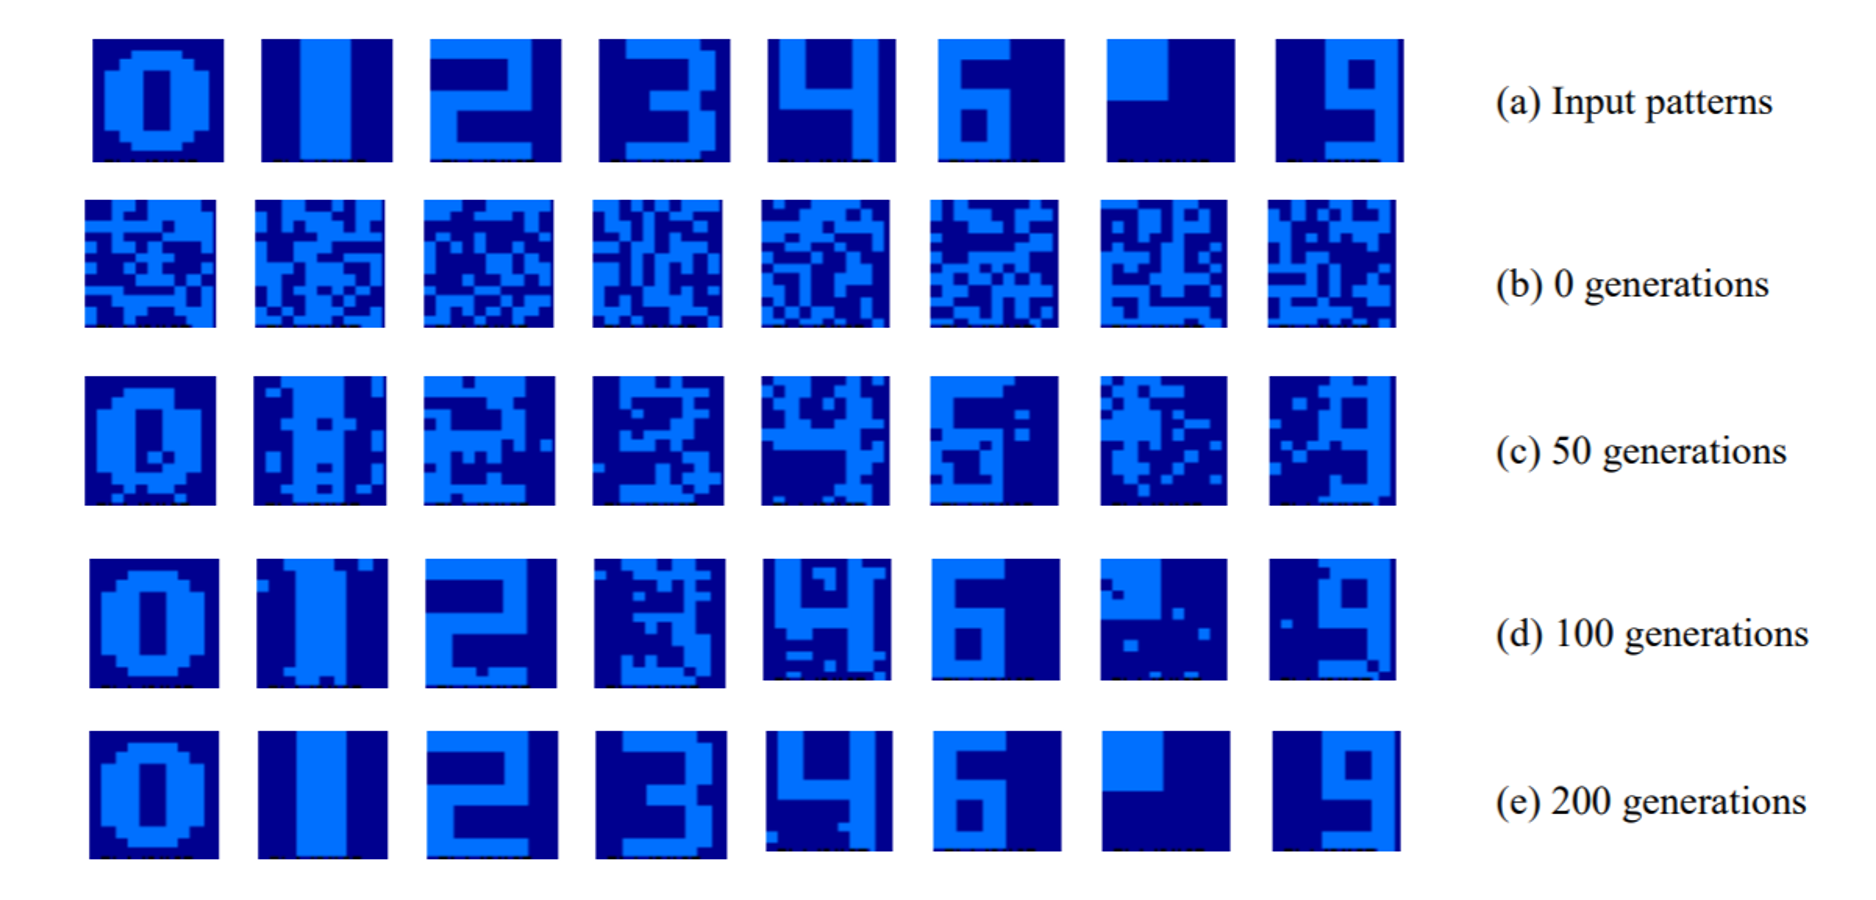
\includegraphics[width=12cm,clip]{images/cj_binary_pattern_learn.png}\\
\caption{Figure 5: Binary Character Recognition.}	
\end{center} 

\subsection{Multi-Modal Optimization}
The CSA reproduces those individuals with higher affinities and selects their improved maturated progenies. This strategy suggests that the algorithm performs a greedy search, where single members will be locally optimized (exploitation of the surrounding space), and the newcomers yield a broader exploration of the searchspace. This characteristic makes the CSA very suitable for solving multi-modal optimization tasks.

Consider the maximizing the function:
\begin{equation} \small{
f(x, y) = x \cdot sin(4 \pi x) - y \cdot sin(4 \pi y + \pi) +1}
 \end{equation}

\begin{center} 
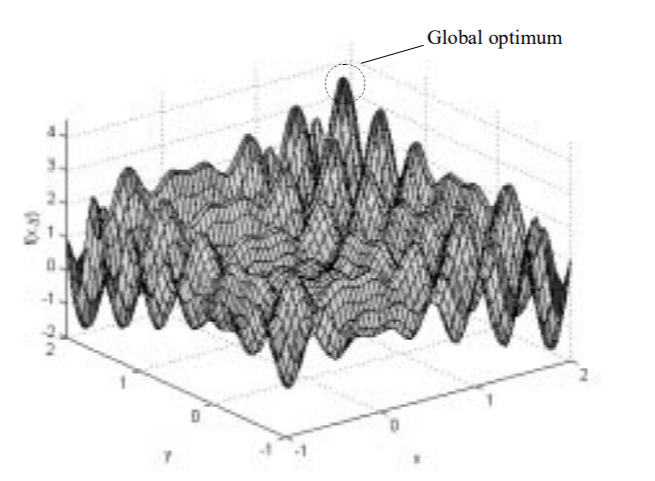
\includegraphics[width=8cm,clip]{images/cj_func_maxi.png}\\
\caption{Figure 6: Function to be maximized by the CSA.}	
\end{center} 

We employed the Hamming shape-space, with binary strings representing real values for \begin{math} x \end{math} and \begin{math} y \end{math}. The chosen bitstring length was \begin{math} L = 22 \end{math},  corresponding to a precision of six decimal places. The variables \begin{math} x \end{math} and \begin{math} y \end{math} are defined over the range \begin{math} [-1, 2]\end{math},  and the mapping from a binary string  \begin{math} m =\left \langle m_L,..., m_2, m_1\right\rangle\end{math} into a real number \begin{math} z \end{math} is completed in two steps:
\begin{itemize}
    \item {convert the binary string \begin{math} m =\left \langle m_L,..., m_2, m_1\right\rangle\end{math} from base 2 to base 10:}
    \begin{equation}\small{(<m_L,..., m_2, m_1>)_2 = (\sum_{i=0}^{21}m_i \cdot 2^i)_{10} \ = \ z^{'}}
    \end{equation}
    \item{find the corresponding real value for \begin{math} z \end{math}:}
    \begin{equation}\small{z=z_{min} + z^{'} \cdot \frac{z_{max} - z_{min}}{2^{22} - 1}, \ where \ z_{max} = 2 \ and \ z_{min} = -1
    }
    \end{equation}
\end{itemize}

The affinity measure corresponds to the evaluation of the
function \begin{math} f(x, y) \end{math} after decoding \begin{math} x \end{math} and \begin{math} y \end{math}, as described above.

The figure below present the  optimized population after 100
generations:
\begin{center} 
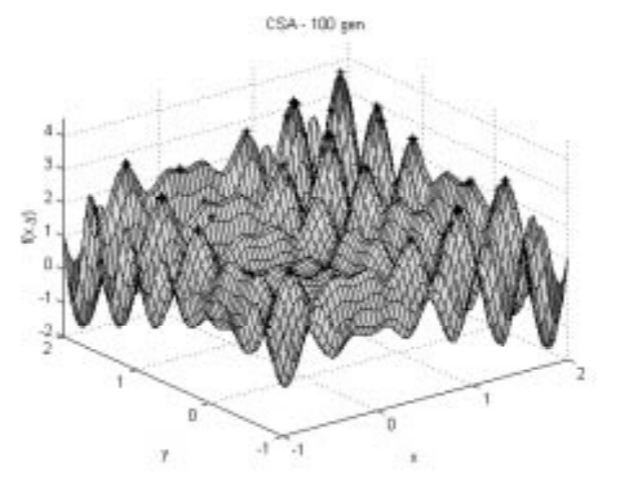
\includegraphics[width=8cm,clip]{images/cj_func_maxi_100.png}\\
\caption{Figure 7: Optimized population after 100 cell generations.}	
\end{center} 

\section{Conclusion}
The clonal selection algorithm was verified to be capable of performing learning and maintenance of high quality memory and, it was also capable of solving complex problems, like multi-modal and combinatorial optimization.


\end{document}
